\def\titulo{Tarea}
\def\subtitulo{Función cuadrática}
\def\curso{Segundo medio}
\documentclass[]{srs2}

\begin{document}

\subsection*{Objetivo}

\subsection*{Instrucciones generales}
Hola.

\subsection*{Ejemplo}

\underline{Problema}: Un granjero desea cercar un terreno rectangular y dispone de
320 [m] de alambre, ¿qué dimensiones debe tener el terreno para que
su área sea máxima?

\underline{Solución}:

Se determinan las dimensiones en términos de una variable.
\begin{columnas}[0.6]
\begin{align*}
  2\left(\text{base}\right) + 2\left(\text{altura}\right) &= \text{perímetro} \\
  2x + 2\left(\text{altura}\right) &= 320 \\
  x + \left(\text{altura}\right) &= 160 \\
  \text{altura} &= 160 - x
\end{align*}
\siguiente
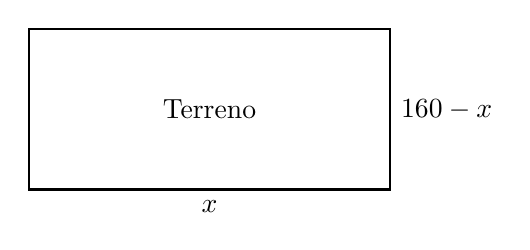
\begin{tikzpicture}
\node[shape=rectangle,inner xsep=1.7cm,inner ysep=0.9cm,
  draw,line width=1pt,name=r] at (0,0) {Terreno};
\node[below] at (r.south) {$x$};
\node[anchor=west] at (r.east) {$160-x$};
\end{tikzpicture}
\end{columnas}
El área es el producto de la base por la altura, se hace el producto y con
esto se obtiene la función \(A\left(x\right)\).
%\begin{center}
%\begin{tblr}{colspec={rcl},cells={mode=math}}
%    A\left(x\right) &=& x(160-x) \\
%  A\left(x\right) &=& 160x - x^2
%\end{tblr}
%\end{center}
\begin{align*}
    A\left(x\right) &= x(160-x) \\
    A\left(x\right) &= 160x - x^2
\end{align*}
La ecuación \(A\left(x\right)\) representa una parábola cóncava hacia
abajo, por lo que el vértice será el punto máximo; esto significa que
el valor de \(x\) en el vértice dará un área máxima.
\begin{equation*}
x = -\dfrac{b}{2a} = - \dfrac{160}{2\left(-1\right)} = -\dfrac{160}{-2} = 80.
\end{equation*}
Así, se deduce que las dimensiones del terreno son de 80 metros
de largo por 80 de ancho. \qed

El problema ya está terminado, pero como nota extra para el alumno,
las coordenadas del vértice son
\(\left(80,\,A\left(80\right)\right) = (80,\, 6.400)\). Donde, 6.400
es el área máxima que puede alcanzar el terreno, y 80 es el largo
del terreno \(\left(x\right)\) que permite alcanzar este valor máximo.

\subsection*{Calculo de la nota}

\begin{equation*}
  \text{Nota final} = \dfrac{d_{f}\cdot n_{f} + d_1 \cdot n_1+d_2 \cdot n_2+\dots+d_n \cdot n_n}{\text{Máximo entre}~\left(25\right)~\text{y}~\left(\text{Dificultad total}\right)~}
\end{equation*}

Donde $d_i$ y $n_i$ corresponden respectivamente a la dificultad del problema
seleccionado y la nota obtenida en dicho problema. $d_f$ y $n_f$ se utilizan
especificamente para evaluar la presentación de la tarea.

\subsection*{Criterios de evaluación}

A continuación presentan los criterios bajo los cuales se evaluará la
presentación de la tarea y la resolución de los problemas.

\subsubsection*{Presentación y formato}
\begin{lista}
* asd asd
* asd asd
* asd asd
\end{lista}
\subsubsection*{Problemas de cálculo}
\begin{lista}
* asd asd
* asd asd
* asd asd
\end{lista}
\subsubsection*{Problemas de planteamiento}
\begin{lista}
* Modela correctamente la problematica. Esto es, expresar la problematica
en terminos matemáticas.
* asd asd
* asd asd
\end{lista}

\begin{center}
  \begin{tblr}{width=\linewidth,colspec={XXX}, hline{1,Z} = {1}{-}{}, hline{1,Z} = {2}{-}{},
      hlines,row{3,5,7}={font={\raggedright\small}},row{2,4,6} = {bg=black!15,halign=c},
      row{1}={halign=c},rows={rowsep=5pt}}
      %%% CABEZERA
      Logrado & Suficiente & Insuficiente \\
      %%% PRESENTACION
      \SetCell[c=3]{c} Presentación (puntaje por informe)& & \\
      La tarea se presenta de forma impecable: letra clara y fácilmente
      legible en todo el documento, sin errores de ortografía.
      El papel está limpio, sin arrugas, dobleces ni manchas. \mbox{(5 puntos)}&
      La tarea es legible en su mayor parte, aunque podría mejorar la claridad
      de la letra en algunas secciones. Presenta errores ortográficos mínimos (1-2)
      y/o pequeñas imperfecciones en el papel (manchas leves, arrugas menores) que no
      dificultan significativamente la lectura. \mbox{(3 puntos)}&
      La letra es difícil de entender en varias secciones, presenta múltiples
      errores de ortografía (3 o más) y/o el papel está descuidado
      (arrugado, manchado, doblado) dificultando la revisión y lectura. \mbox{(0 puntos)}\\
      %%% PROCESOS Y JUSTICACACION
      \SetCell[c=3]{c} Procesos y justificación (puntaje por pregunta) & & \\
      Detalla cada paso del procedimiento de forma clara, ordenada y sistemática.
      Justifica adecuadamente las operaciones, propiedades o estrategias matemáticas
      utilizadas, demostrando una comprensión profunda del problema y cómo se alcanza
      la solución. El razonamiento es fácil de seguir. \mbox{(3 puntos)}&
      Presenta la mayoría de los pasos del procedimiento, aunque algunos podrían ser
      más detallados o claros. La justificación es adecuada en general, pero puede
      haber omisiones menores o falta de precisión en alguna explicación.
      El proceso general es comprensible, aunque con algunas dificultades para
      seguir el razonamiento en puntos específicos. \mbox{(2 puntos)}&
      Los pasos del procedimiento son confusos, incompletos, desordenados o ausentes.
      La justificación es escasa, ausente o incorrecta. No es posible seguir el
      razonamiento para entender cómo se intentó llegar al resultado. \mbox{(0 puntos)}\\
      %%% RESULTADOS
      \SetCell[c=3]{c} Resultados (puntaje por pregunta)& & \\
      El resultado alcanzado es correcto y está desarrollado completamente, es decir,
      no se dejaron valores expresados y/o sin simplificar. \mbox{(3 puntos)} &
      El resultado está casi correcto. El error es aritmético y no conceptual,
      o simplemente falto desarrollar la respuesta. \mbox{(2 puntos)}&
      El resultado no responde de ninguna manera al enunciado y/o hay errores que
      son fundamentales. \mbox{(0 puntos)}\\
  \end{tblr}
\end{center}

\end{document}